%!TEX program = xelatex

\documentclass[a4paper, openany, oneside]{memoir}
\usepackage[no-math]{fontspec}
\usepackage{pgfplots}
\pgfplotsset{compat=newest}
\usepackage{commath}
\usepackage{mathtools}
\usepackage{amssymb}
\usepackage{amsthm}
\usepackage{booktabs}
\usepackage{mathtools}
\usepackage{xcolor}
\usepackage[separate-uncertainty=true, per-mode=symbol]{siunitx}
\usepackage[noabbrev, capitalize]{cleveref}
\usepackage{listings}
\usepackage[american inductor, european resistor]{circuitikz}
\usepackage{amsmath}
\usepackage{amsfonts}
\usepackage{ifxetex}
\usepackage[dutch,english]{babel}
\usepackage[backend=bibtexu,texencoding=utf8,bibencoding=utf8,style=ieee,sortlocale=en_GB,language=auto]{biblatex}
\usepackage[strict,autostyle]{csquotes}
\usepackage{parskip}
\usepackage{import}
\usepackage{standalone}
\usepackage{hyperref}
%\usepackage[toc,title,titletoc]{appendix}

\ifxetex{} % Fonts laden in het geval dat je met Xetex compiled
    \usepackage{fontspec}
    \defaultfontfeatures{Ligatures=TeX} % To support LaTeX quoting style
    \setromanfont{Palatino Linotype} % Tover ergens in Font mapje in root.
    \setmonofont{Source Code Pro}
\else % Terug val in standaard pdflatex tool chain. Geen ondersteuning voor OTT fonts
    \usepackage[T1]{fontenc}
    \usepackage[utf8]{inputenc}
\fi
\newcommand{\references}[1]{\begin{flushright}{#1}\end{flushright}}
\renewcommand{\vec}[1]{\boldsymbol{\mathbf{#1}}}
\newcommand{\uvec}[1]{\boldsymbol{\hat{\vec{#1}}}}
\newcommand{\mat}[1]{\boldsymbol{\mathbf{#1}}}
\newcommand{\fasor}[1]{\boldsymbol{\tilde{\vec{#1}}}}
\newcommand{\cmplx}[0]{\mathrm{j}}
\renewcommand{\Re}[0]{\operatorname{Re}}
\newcommand{\Cov}{\operatorname{Cov}}
\newcommand{\Var}{\operatorname{Var}}
\newcommand{\proj}{\operatorname{proj}}
\newcommand{\Perp}{\operatorname{perp}}
\newcommand{\col}{\operatorname{col}}
\newcommand{\rect}{\operatorname{rect}}
\newcommand{\sinc}{\operatorname{sinc}}
\newcommand{\IT}{\operatorname{IT}}
\newcommand{\F}{\mathcal{F}}

\newtheorem{definition}{Definition}
\newtheorem{theorem}{Theorem}


\DeclareSIUnit{\voltampere}{VA} %apparent power
\DeclareSIUnit{\pii}{\ensuremath{\pi}}

\hypersetup{%setup hyperlinks
    colorlinks,
    citecolor=black,
    filecolor=black,
    linkcolor=black,
    urlcolor=black
}

% Example boxes
\usepackage{fancybox}
\usepackage{framed}
\usepackage{adjustbox}
\newenvironment{simpages}%
{\AtBeginEnvironment{itemize}{\parskip=0pt\parsep=0pt\partopsep=0pt}
\def\FrameCommand{\fboxsep=.5\FrameSep\shadowbox}\MakeFramed{\FrameRestore}}%
{\endMakeFramed}

% Impulse train
\DeclareFontFamily{U}{wncy}{}
\DeclareFontShape{U}{wncy}{m}{n}{<->wncyr10}{}
\DeclareSymbolFont{mcy}{U}{wncy}{m}{n}
\DeclareMathSymbol{\Sha}{\mathord}{mcy}{"58}
\addbibresource{../../../includes/bibliography.bib}

\title{Introduction}

\author{W.P. Bruinsma \and R.P. Hes \and H.J.C. Kroep \and T.C. Leliveld \and W.M. Melching \and T.A. aan de Wiel}

\raggedbottom

\begin{document}

\section{General description}
Our system is an approach which enables real-time high-performance wideband spectrum sensing. The goal of our system is to determine which frequencies of a signal contain signals distinct from noise. To achieve this goal, we will divide our system into several modules which all work together. Each module will be specified and designed separately.

Determining whether a signal is distinct from noise forms a decision problem. To evaluate this problem, one could reconstruct the spectrum of the signal, and determine whether it resembles one of noise. However, it can be shown that the decision problem is solved optimally by evaluating the signal power \cite{axell2012spectrum}. Therefore, we could look at the signal power per frequency to decide per frequency whether a signal present or not. The signal power per frequency is also called the power spectral density. But it turns out that the power spectral density is derived from the spectrum of a signal, and requires less information than reconstruction of the spectrum would. Therefore, we focus on an approach which is centered around the reconstruction of the power spectral density.

The first step in high-performance real-time wideband spectrum sensing is sampling the signal whose spectrum has to be sensed. Conventionally, this is done by making use of uniform sampling at the Nyquist frequency\footnote{The Nyquist frequency is the minimum frequency at which a signal can be sampled without distorting the signal. The Nyquist frequency is twice the highest frequency present in the signal.}. This ensures that the signal can be reconstructed after sampling. However, the Nyquist frequency becomes high when one wants to sense a large bandwidth. As a consequence, expensive hardware must be used. Clearly, we must look for alternatives. To do this, we investigate sampling techniques which differ from uniform sampling.

So far, we have not specified what system actually consists of. Concretely, we will design a mathematical framework. This framework will be made of many existing methods and theories, and will form the theoretical basis of the toolkit described in the introduction. Since we design a mathematical framework, our specifications will be mostly functional, and less quantative. 

% These techniques can be implemented by making use of multiple sampling devices, also called samplers. Non-uniform sampling is discussed in \cref{cha:sampling} and non-uniform sampling techniques are discussed in \cref{cha:sampling_methods}.


% Spectrum sensing consists of determining which frequencies of a signal are occupied with signals distinct from noise. Our approach, which we consider to be a system, enables to determine these frequencies. Therefore, the input to our system consists of an arbitrary signal and the output is which frequencies of this signal are occupied by signals distinct from noise. We will not only consider signals from a single source, but also consider the same signal observed by multiple sources. These sources all observe the same signal by sampling this signal. So, in summary, our system will be able to combine the information obtained by a single or multiple sources all sampling the sample signal, and will then be able to determine which frequencies of this signal are occupied by signals distinct from noise.

% In this part, we develop an approach to enable high-performance real-time wideband spectrum sensing. The part is divided into several chapters. We start with a detailed description of the approach. Then, we give an overview of the system. In this overview, we look at the different system components, which will be described in separate chapters afterwards. Finally, we will evaluate the system as a whole.

\section{System specification}
\label{sec:theory-specs}
Now that we have identified our goal, we will proceed to describe our system in a detailled manner. This description consists of specifications according to which our system will be designed. The specifications are divided into several categories. The categories are then analysed by MoSCoW prioritisation.

As stated in the introduction, the goal of our system is to determine which frequencies are occupied. However, some signals resemble noise very closely. We therefore do not require that we recognise such signals. In addition, we do not require that we can sense an infinitely large bandwidth. In summary, our system \emph{must} enable spectrum sensing such that the application
\begin{enumerate}
    \item is able to identify at which frequencies signals are present, where signals
    \begin{enumerate}
        \item can be any signal distinct from noise and
        \item can have any reasonable signal strength;
    \end{enumerate}
    \item is able to sense any reasonably sized bandwidth and
    \item the spectrum sensing is done in real-time.
\end{enumerate}
In addition, our system \emph{should} enable spectrum sensing such that the application
\begin{enumerate}
    \item is able to sense very large bandwidths and
    \item the spectrum sensing is done as efficient as possible.
\end{enumerate}

\subsection{Detection}
We have described the functionality of our system on a high level. However, distincting signals from noise, which from now on we refer to as the detection of signals, requires a little more care. Ideally, we want to specify how accurate we can identify the frequencies which are occupied. Also, since wideband spectrum sensing is not considered solved, we want to know how accurate our detection is.
In summary, detection of signals \emph{must} be such that
\begin{enumerate}
    \item detection of signals consists of determination of the set of frequencies which are occupied by signals other than noise;
    \item the resolution of these frequencies can be specified and
    \item the correctness of operation can be specified.
\end{enumerate}
In addition, detection of signals \emph{should} be such that
\begin{enumerate}
    \item the resolution of detection can be as high as possible;
    \item its operation can be as correct as possible and
    \item its operation is as efficient as possible.
\end{enumerate}

\subsection{Sampling techniques}
We discussed that the first step in spectrum sensing is sampling the signal whose spectrum has to be sensed. It turned out that sampling at the Nyquist frequency is not efficient enough. We would therefore like to design efficient sampling techniques, which can distribute the workload across multiple devices. In summary the techniques used for sampling \emph{must} allow for
\begin{enumerate}
    \item correct operation of the detection;
    \item usage of a single sampling device and
    \item usage of multiple sampling devices such that the workload can be distributed across the devices.
\end{enumerate}
In addition, the sampling techniques \emph{should} allow for
\begin{enumerate}
    \item sampling as efficient as possible.
\end{enumerate}

\subsection{Reconstruction}
After the signal is sampled, the obtained information must be processed such that detection is possible. We already argued that is done most efficiently by the reconstructing the power spectral density, which must be done real-time. Also, this reconstruction must be as accurate as possible. In summary, the \textit{reconstruction} must allow for
\begin{enumerate}
    \item corrected operation in conjunction with the sampling techniques and
    \item real-time operation.
\end{enumerate}
In addition, the \textit{reconstruction} should be
\begin{enumerate}
    \item as efficient as possible and
    \item as fast as possible.
\end{enumerate}



% Compressive sensing is a subject that has made some important improvements in recent years. D.Ariananda and G.Leus published a paper in 2012 that proposed a new method in compressive sampling. When calculating the power spectral density of a signal, a lot of information is lost during the process. This paper exploits this fact by sampling in such a way, that only the information required to calculate the power spectral density is acquired. This allows for much less samples than Nyquist.

% Compressive sensing is an active area of research \textbf{meer}. Most algorithms are based on L1-techniques and try to recover the spectrum of the signal, and therefore assume that the signal is \emph{sparse} in the Fourier domain. Recent developments \textbf{papers van leus en ariananda hier} have shown that it is possible to reconstruct the power spectral density instead of the spectrum without the assumption of sparsity.

% This thesis targets a accessible theoretical description of the compressive sensing system implemented during

% Main product: Extendable Toolkit for High-Performance Spectrum Sensing

% methode om high-performance te spectrum sensen



% Method which describes

% - spectrum sensing
% - psd
% - detection
% - sampling methods
% - high-performance
% - real-time



% - uitleg hoofdstukken
% - kort systeemoverzicht + tikz
\section{System overview}
\label{sec:theory-system-overview}
Our system consists of several components, which all work together to achieve the functionality specified in the previous section. The components are as follows.

\begin{description}
    \item[Sampling] Sampling consists of applying various sampling techniques to the signal whose spectrum has to be sensed. The actual sampling is not part of the system, but forms an interface between the the signal and our system.
    \item[Reconstruction] Reconstruction analyses the sampled signal and tries to reconstruct the power spectral density. Reconstruction has knowledge of the used sampling technique to perform its operation.
    \item[Detection] Detection performs the identification of signals based on the analysis of the reconstruction. Detection and reconstruction closely work together.
\end{description}

The modules are depicted in \cref{fig:overview}.
\begin{figure}
    \centerline{
    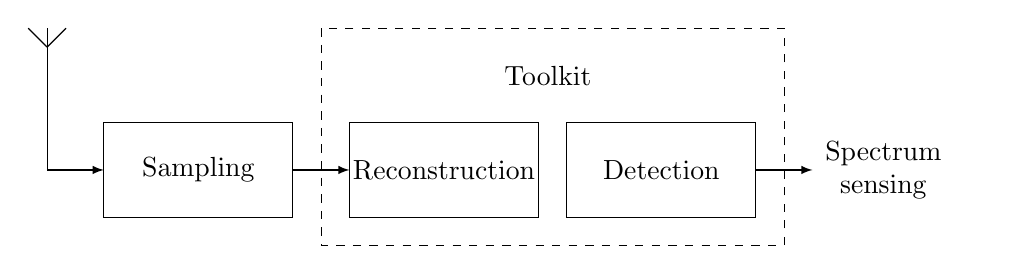
\begin{tikzpicture}[scale=1.2]
    \draw  (-0.6,1.5) rectangle (1.4,0.5) node[pos=.5]{Sampling};
    \draw  (2,1.5) rectangle (4,0.5) node[pos=.5]{Reconstruction};
    \draw  (4.3,1.5) rectangle (6.3,0.5) node[pos=.5]{Detection};
    \draw  [white] (6.9,1.5) rectangle (8.9,0.5) node[pos=.5,text width=2cm, align=center,black,xshift=-0.3cm]{\centering Spectrum sensing};
    \draw  [dashed] (1.7,2.5) rectangle (6.6,0.2);
    \node at (4.1,2) {Toolkit};
    \draw [>=latex,->] (1.4,1) -- (2,1);
    \draw [>=latex,->] (6.3,1) -- (6.9,1);
    \draw [>=latex,->] (-1.2,1) -- (-0.6,1);
    \draw (-2+0.8,1) -- (-2+0.8,2.5);
    \draw (-1.8+0.8,2.5) -- (-2+0.8,2.3);
    \draw (-2.2+0.8,2.5) -- (-2+0.8,2.3);
    \end{tikzpicture}}
    \caption{System overview. The system components are shown.}
    \label{fig:overview}
\end{figure}

In summary, the signal whose spectrum had to be sensed is first sampled. Then its power spectral density is reconstructed by means of algorithms designed for the sampling techniques. Detection then analyses this power spectral density, and decides per frequency whether a signal is present or not. This decision process is not based upon which kind of information is encoded in those frequencies, but only determines if \textit{any} kind of information is present. After it is determined at which frequencies signals are present, the spectrum sensing process is complete.

\cref{cha:sampling} will give an introduction to non-uniform sampling. Then \cref{cha:reconstruction} will describe a way to reconstruct a power spectral density. Afterwards, different sampling techniques will be considered in \cref{cha:sampling_methods}. \cref{cha:detection} will discuss how this power spectral density is used for detection. Finally, we will evaluate our system in \cref{cha:system_evaluation_theory} and discuss the obtained results in \cref{cha:discussion_theory}.

\end{document}